% Learning through Discernment. Compile with pdflatex + bibtex (e.g. latexmk -pdf main.tex), or on Overleaf.
\documentclass[11pt]{article}
\usepackage[utf8]{inputenc}
\usepackage[T1]{fontenc}
\usepackage[margin=1in]{geometry}
\usepackage{lmodern}
\usepackage{amsmath,amssymb}
\usepackage{graphicx}
\usepackage{booktabs,longtable,array,calc}
\usepackage[numbers,sort&compress]{natbib}
\usepackage{xcolor}
\usepackage[colorlinks=true,linkcolor=blue!50!black,citecolor=blue!50!black,urlcolor=blue!50!black]{hyperref}
\usepackage{fvextra}
\usepackage[section]{placeins}  % floats stay within their own section
\providecommand{\tightlist}{\setlength{\itemsep}{0pt}\setlength{\parskip}{0pt}}
\fvset{fontsize=\small}
\RecustomVerbatimEnvironment{verbatim}{Verbatim}{breaklines=true,fontsize=\small,frame=single}
\setlength{\emergencystretch}{3em}

\title{Learning through Discernment: when a small language model learns from user feedback on the job, and when it decays}
\author{Sirisilp Kongsilp\\[2pt]
\small Decentralized Science, Inc.\\
\small Department of Computer Engineering, Kasetsart University\\
\small \texttt{tai@kratai.com}, \texttt{sirisilp.k@ku.th}}
\date{Draft, November 2026}

\begin{document}
\maketitle
\begin{abstract}
Small language models deployed on a device could keep improving by learning from their own work, but only if something decides which experiences are worth learning from. We study this in a ``creature'': a frozen Qwen3 model (0.6B or 1.7B) with a small LoRA adapter that works by day and, each night, trains on the episodes judged good, replaying recent lessons. Over lives of up to 60 days we compare judges modelled on published approaches: the model's own judgment (as in self-rewarding models), its reflection on the user's reaction, the user's stated verdict read without error, a separate frozen ``feedback sense'' model that reads the reaction, and an oracle that knows the true outcome (as in training on verified successes).

On WebShop, learning from its own judgment decayed in every life, while the oracle improved and then held steady for 60 days. A first feedback sense (v2) let a few polite give-ups through as successes, and 3 of 5 lives collapsed after learning from them on the first night. A second (v3), built for discernment, which first asks whether the user gave a clear verdict at all, cut the reactions it misread as approval from 5.0\% to 1.2\%, and 4 of 5 lives reached near-oracle scores within 14 days. They then declined slowly, although their lessons stayed clean: about 2 a day against the oracle's 20, with only 2-10\% failures. Across 97 lives, the share of failed attempts among a life's lessons predicted where it ended (Spearman $\rho$ = -0.81): a handful of correct lessons was enough to improve, and a handful of wrong ones enough to collapse.

On $\tau^2$-bench, where a simulated customer cannot see whether its request was actually carried out, 80\% of the lessons sense v3 accepted were failed tasks, and all three 1.7B sense v3 lives collapsed within 30 days. Even oracle lessons did not raise overall scores: they came mostly from the easiest domain, which improved while the other learned domain and a never-practised one declined.

Learning from users works only when the judge keeps failed attempts out of the lessons, which needs users who can see the outcome; and even correct lessons must be balanced across skills to avoid forgetting.
\end{abstract}

\section{Introduction}

The introduction argues that on-device models need a way to learn on the job, that the hard part is deciding what to learn from, and that we measure this over long lives rather than single updates.

\begin{itemize}
\tightlist
\item
  \textbf{Motivation:} small models on phones and devices meet new tasks after release; retraining in the cloud is costly and slow. A model that improves from its own daily work would close that gap.
\item
  \textbf{The core problem:} learning on the job needs a judge of which episodes were good. Without a true outcome, the options are the model's own judgment or the user's reaction, and both can be wrong.
\item
  \textbf{The gap:} most work measures one round of improvement on a fixed benchmark. Little measures what happens over weeks of nightly updates, where small errors in the judge compound.
\item
  \textbf{Our approach:} a ``creature'' that works by day and sleeps on its lessons at night, run for 14 days to a year under different judges, including a separate frozen model, the feedback sense, that reads the user's reaction. We call what it must provide discernment: telling an informed, clear verdict on the result from a polite, vague or uninformed reaction. The other judges are simplified versions of published approaches, compared with it under the same model, tasks and training budget.
\item
  \textbf{Contributions:}

  \begin{enumerate}
  \def\labelenumi{\arabic{enumi}.}
  \tightlist
  \item
    A long-horizon test of nightly self-training for small models, on WebShop and $\tau^2$-bench, with an oracle as the upper bound.
  \item
    Evidence that learning from the model's own judgment decays, and that what decides a life is the share of failed attempts among its lessons, not their number ($\rho$ = -0.81 across 97 lives): a few accepted give-ups can collapse a life.
  \item
    A feedback sense with discernment, which first asks whether the user gave a clear verdict. It removes most bad lessons and reaches near-oracle scores for two weeks, then fades for reasons we leave open.
  \item
    Evidence that learning from reactions fails when users cannot see the outcome, and that even correct but lopsided lessons cause forgetting.
  \end{enumerate}
\end{itemize}

\section{Related work}

We place the work where continual learning, learning from feedback and self-training meet. References to collect: {[}to do{]}.

\begin{itemize}
\tightlist
\item
  \textbf{Continual learning and forgetting:} replay, regularisation (for example EWC) and parameter-efficient adapters such as LoRA; most studies use labelled task streams, not unlabelled daily work.
\item
  \textbf{Learning from human feedback:} RLHF and DPO learn from explicit preference labels collected offline; we learn from implicit reactions online.
\item
  \textbf{Self-training and self-reward:} models that judge or reward their own outputs; known to drift and to reward-hack, which our self-judging lives reproduce.
\item
  \textbf{Learning from user reactions:} work on implicit feedback in dialogue, and MemoryBench (learning from user feedback, ICML 2026).
\item
  \textbf{Agent benchmarks with simulated users:} $\tau$-bench and $\tau^2$-bench, WebShop; the gap between what a user sees and the true outcome.
\item
  \textbf{To write: why no direct comparison with published results.} The published methods behind our judges (STaR, self-rewarding models, Reflexion, learning from implicit feedback) were tested over one round of improvement, not over weeks of nightly updates. No long-life results exist to compare against, so we run simplified versions in one shared loop; say this is a deliberate control, not a shortcut.
\item
  \textbf{To write: the two ``sleep'' papers} (Language Models Need Sleep, arXiv 2606.03979; Do Language Models Need Sleep?, CMU/UMD): they study how memories are consolidated, given the lessons; we study who decides what the lessons are.
\end{itemize}

\section{The creature}

We call the system a creature: a small language-model agent that works by day and is fine-tuned at night (its ``sleep'') on lessons chosen by a judge. These names label an ordinary continual fine-tuning loop; they make no claim about biology. Its base model never changes; everything it learns lives in a small LoRA adapter, trained each night on the day's lessons (Fig.~\ref{fig:1}).

\begin{figure}[htbp]
\centering
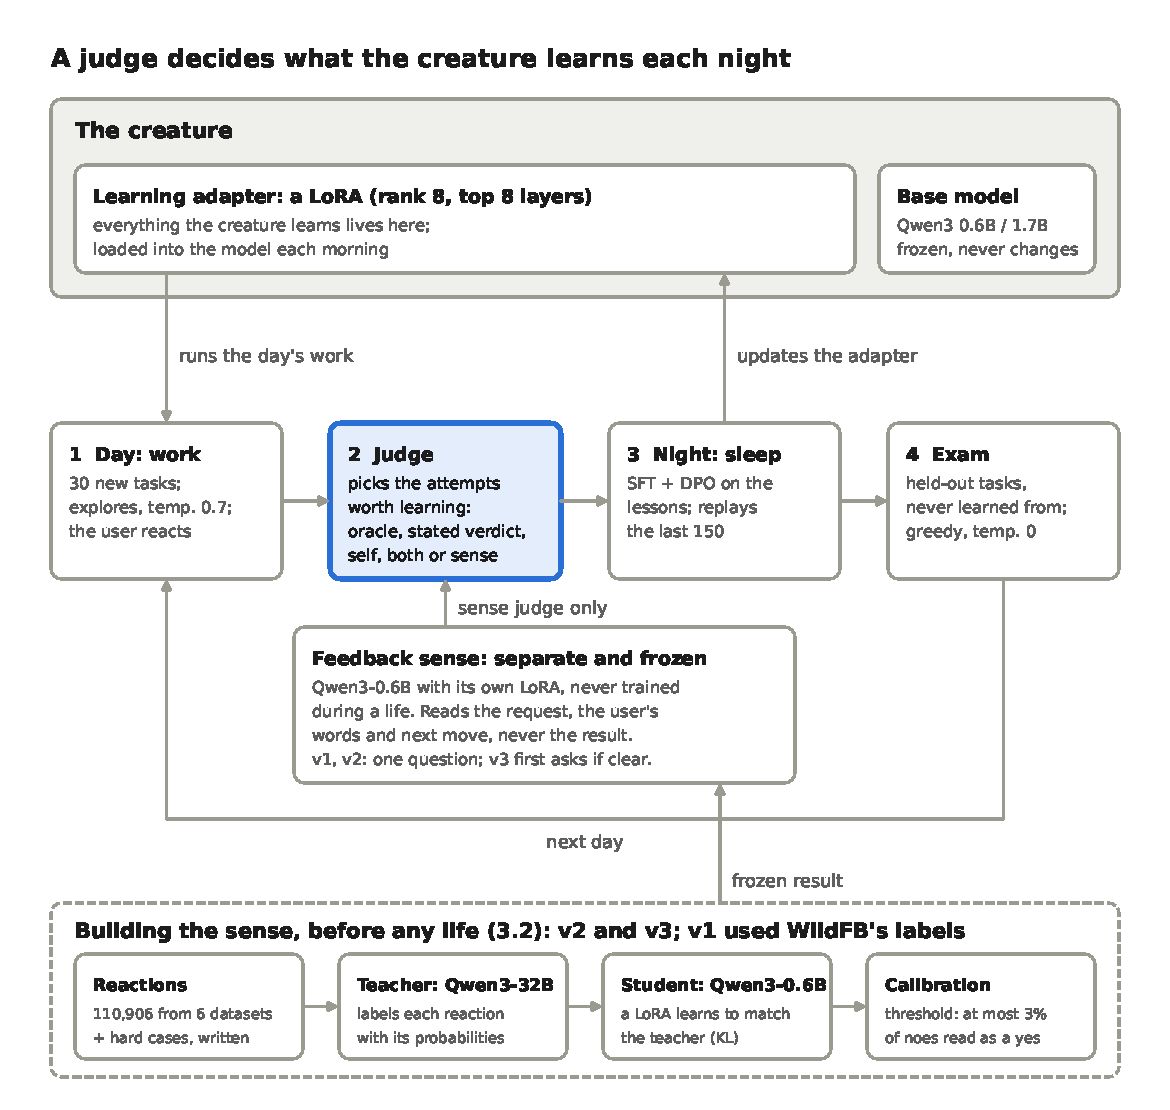
\includegraphics[width=0.9\linewidth]{figures/fig1_creature}
\caption{The creature's parts (top), its daily cycle (middle), the feedback sense (bottom) and how the sense was built, once, before any life (dashed); the judge, highlighted, is what the experiments vary}
\label{fig:1}
\end{figure}

\subsection{The daily cycle}

\textbf{Body.} A frozen Qwen3 \cite{yang2025qwen3} base model (Fig.~\ref{fig:1}, top right), 0.6B or 1.7B parameters, served with vLLM \cite{kwon2023vllm} with thinking mode off. Each turn the agent replies in JSON with a short thought, an action and its input, as ``a personal assistant for one user''. The learning adapter (Fig.~\ref{fig:1}, top left) is a LoRA \cite{hu2022lora} of rank 8 on the attention and feed-forward projections of the top 8 layers, loaded into vLLM at run time so each morning's creature uses the previous night's adapter.

\textbf{Day.} In the first step of each day (Fig.~\ref{fig:1}, step 1), the creature works through a fixed number of new tasks (30 a day in every experiment), sampling at temperature 0.7 so it explores. After each attempt the simulated user reacts in words. The true outcome is logged for analysis, but the creature sees it only when the \emph{oracle} is its judge.

\textbf{Judge.} A judge then decides which attempts become lessons (Fig.~\ref{fig:1}, step 2, highlighted because it is the one part the experiments vary). We compare five (Table~\ref{tab:3}), each a simplified stand-in for a published family of methods.

\begin{longtable}[]{@{}
  >{\raggedright\arraybackslash}p{(\linewidth - 6\tabcolsep) * \real{0.2500}}
  >{\raggedright\arraybackslash}p{(\linewidth - 6\tabcolsep) * \real{0.2500}}
  >{\raggedright\arraybackslash}p{(\linewidth - 6\tabcolsep) * \real{0.2500}}
  >{\raggedright\arraybackslash}p{(\linewidth - 6\tabcolsep) * \real{0.2500}}@{}}
\caption{The judges. Only the sense condition uses the feedback sense.}\label{tab:3}\tabularnewline
\toprule\noalign{}
\begin{minipage}[b]{\linewidth}\raggedright
Judge
\end{minipage} & \begin{minipage}[b]{\linewidth}\raggedright
Who decides
\end{minipage} & \begin{minipage}[b]{\linewidth}\raggedright
What it sees
\end{minipage} & \begin{minipage}[b]{\linewidth}\raggedright
Stands in for
\end{minipage} \\
\midrule\noalign{}
\endfirsthead
\toprule\noalign{}
\begin{minipage}[b]{\linewidth}\raggedright
Judge
\end{minipage} & \begin{minipage}[b]{\linewidth}\raggedright
Who decides
\end{minipage} & \begin{minipage}[b]{\linewidth}\raggedright
What it sees
\end{minipage} & \begin{minipage}[b]{\linewidth}\raggedright
Stands in for
\end{minipage} \\
\midrule\noalign{}
\endhead
\bottomrule\noalign{}
\endlastfoot
\emph{oracle} & the benchmark's own score: reward 0.5 or more (WebShop), a full pass ($\tau^2$-bench) & the true outcome & training only on verified successes (STaR \cite{zelikman2022star}, rejection-sampling fine-tuning \cite{yuan2023scaling}); an upper bound no deployed system has \\
\emph{stated verdict} (``\emph{stated}'' in figures) & a fixed rule, no model & the kind of reaction the simulated user chose to give, not its words: praise or ``perfect'' is a yes; silence, settling or moving on is nothing; anything else is a no & learning from explicit user feedback, read without error; an ideal no deployed system has \\
\emph{self} & the creature itself, reflecting on its attempt & its own steps and what it bought; not the user's reaction & self-rewarding models \cite{yuan2024selfrewarding} \\
\emph{both} & the creature itself, reflecting on its attempt & its own steps, what it bought, and the user's words & Reflexion-style reflection with outside feedback \cite{shinn2023reflexion} \\
\emph{sense} & a separate, frozen model (3.2) & the request and the user's next move and words; never the result & our proposal \\
\end{longtable}

\emph{Self} and \emph{both} are the same model with the same prompt; only \emph{both} has the user's reaction in its prompt; \emph{self} is told the user said nothing. The \emph{stated verdict} is not a cruder sense but its ceiling: what a reader of reactions would achieve if it never misread one. With the plain user of Experiment 1, which says ``perfect'' only after a fully correct purchase (reward 1) and stays silent 20\% of the time, the \emph{stated verdict} accepts fewer attempts than the \emph{oracle} and never a failure. Experiment 1 also has a life with no judge and no sleep (\emph{none}).

Where the benchmark allows it, an attempt judged bad gets one retry, and a successful retry becomes a lesson and a preference pair (Section 4). None of the judges is the original implementation of its method; each is the simplest version that fits the same nightly loop, so differences between conditions come from the judge alone.

\textbf{Night.} At night (Fig.~\ref{fig:1}, step 3) the adapter, and only the adapter, is trained on the lessons with supervised fine-tuning, plus DPO \cite{rafailov2023dpo} ($\beta$ = 0.1) on the preference pairs. Learning rate 1e-4, 2 epochs, at most 40 steps a night. Each night replays the 150 most recent lessons, so old lessons fade out as new ones arrive. A lesson's loss is spread across its steps, so a 15-step attempt counts as much as a 3-step one (in the sleep variant of Experiment 3 and in Experiments 4 and 5; earlier, each step counted as a lesson of its own).

\textbf{Exams.} The exam (Fig.~\ref{fig:1}, step 4) uses fixed held-out tasks, never learned from, attempted greedily (temperature 0): every morning on WebShop, every 3 days on $\tau^2$-bench, and on day 0 before any learning. The next day starts with the adapter that night produced (the loop along the bottom of Fig.~\ref{fig:1}), so each day's work uses everything learned so far.

\subsection{The feedback sense}

The sense (Fig.~\ref{fig:1}, bottom) is the creature's source of discernment, and is used only in the sense condition: a second, frozen Qwen3-0.6B with its own LoRA (rank 16), served beside the creature and never trained during a life. It reads three things: the user's request, the kind of move the user made next (replied, made a new request, asked to adjust, repeated the request, left, said nothing) and the user's words. It never sees what the creature did or how it turned out, so it reads people rather than judging the work. Because the sense is frozen and separate, the creature cannot change how it is judged.

\emph{Answers.} The sense gives one of five answers: 100 (exactly right), 80 (acceptable, or good enough to build on), 20 (one part missed what was asked), 0 (wrong) or null (unclear); Table~\ref{tab:4} gives examples. They form two groups with a gap between them: 100 and 80 are a yes, 20 and 0 are a no, and there is no middle score. A reaction that does not clearly belong to one side is null, and nothing is learned from it. The gap is deliberate. The creature should learn only from a clear signal, so the sense must commit to a side or abstain, rather than hand the judge a lukewarm 50 to round one way or the other. Null comes about in three ways: the reaction says nothing about the result (silence, ``hmm'', settling, leaving without a word); the sense is not confident enough of its answer (under the threshold set in calibration); or, in v3 (below), the reaction is not a clear verdict at all. Each answer begins with a different token (0, 2, 8, 1, n), so the sense decides in one forward pass, and its confidence is the probability of that first token.

A yes makes the attempt a lesson; an 80 counts half, since ``fine, next'' says less than praise. A no is not wasted on WebShop: it triggers the retry described in Section 4, with a hint matched to the answer, and if the sense reads the user's reaction to the retry as a yes, the retry becomes a lesson and a preference pair. On $\tau^2$-bench, which has no retry, a no teaches nothing.

\emph{Data.} We built the sense by distillation \cite{hinton2015distilling}, from conversations unrelated to our tests. Its raw material is 110,906 moments from six public datasets where an assistant delivered something and the user's next turn shows how they took it: WildFB \cite{peng2026wildreward} and WildFeedback \cite{shi2026wildfeedback} (30,000 each, both drawn from WildChat \cite{zhao2024wildchat}), Taskmaster 1-3 \cite{byrne2019taskmaster} (20,000), MultiWOZ 2.2 \cite{zang2020multiwoz} and ReDial \cite{li2018redial} (15,000 each) and CCPE-M \cite{radlinski2019ccpe} (906; Table~\ref{tab:A3}). Turns where the assistant only asked a question were skipped, since the answer is not a reaction, and shopping was left out, since it is the test domain. Real data rarely holds the hard cases, so the teacher also wrote 4,728 reactions of eight kinds (politely unhappy, settling, vague, sarcastic, ``not my style'', firm rejection, building on the result, plain acceptance) across ten task types and six personas, chosen to differ from our WebShop user's.

\emph{Teacher.} Qwen3-32B labelled every reaction under a written guide. It saw the assistant's reply as context; the student never does. Instead of one label we kept the teacher's probabilities over the five answers, read from the log-probabilities of its first answer token, so the student learns the teacher's doubt as well as its choice. On the two datasets that carry their own signal of success, the teacher agreed with it on yes or no 81\% (WildFB) and 85\% (WildFeedback) of the time, and it called about half of the WildFB reactions unclear. The teacher is not a perfect reader either (Fig.~\ref{fig:8}a). Of the reactions it wrote itself, it read half of the politely unhappy and half of the sarcastic ones as a yes, a quarter of the settling ones, and 16\% of warm thanks for trying, a kind added for v3 (below). The student inherits these mistakes; the confidence threshold below, and v3's question about a clear verdict, are what is meant to keep them out of the creature's lessons.

\emph{Student and calibration.} The student learns to match the teacher's probabilities (KL divergence) on 47,800 reactions, balanced so that no task type or answer dominates, for one epoch (learning rate 1e-4, batch 16, under an hour on one GPU). In half the training rows the request is hidden, so the sense must rely on the reaction itself. After training, a temperature is fitted on 2,000 held-out reactions, and a confidence threshold is chosen as the lowest that keeps false accepts (a no read as a yes) at or under 3\%; below it, the sense answers null. This is sense v2 (an earlier v1, trained on one dataset's own labels, was replaced before the experiments reported here). Its threshold is 0.65. On the held-out reactions it gave a verdict on 30\% of them, agreed with the teacher's side on 92\% of those, and read 2.9\% of the teacher's noes as a yes. Trained nine more times, each time without one task type and tested on it, it read 0.5-8.1\% of the unseen type's noes as a yes (Fig.~\ref{fig:8}b). Four types stayed under the 3\% target and three barely passed it; writing (6.9\%) and booking and ordering (8.1\%), the type closest to shopping, did not. A new kind of task can loosen the sense.

\begin{figure}[htbp]
\centering
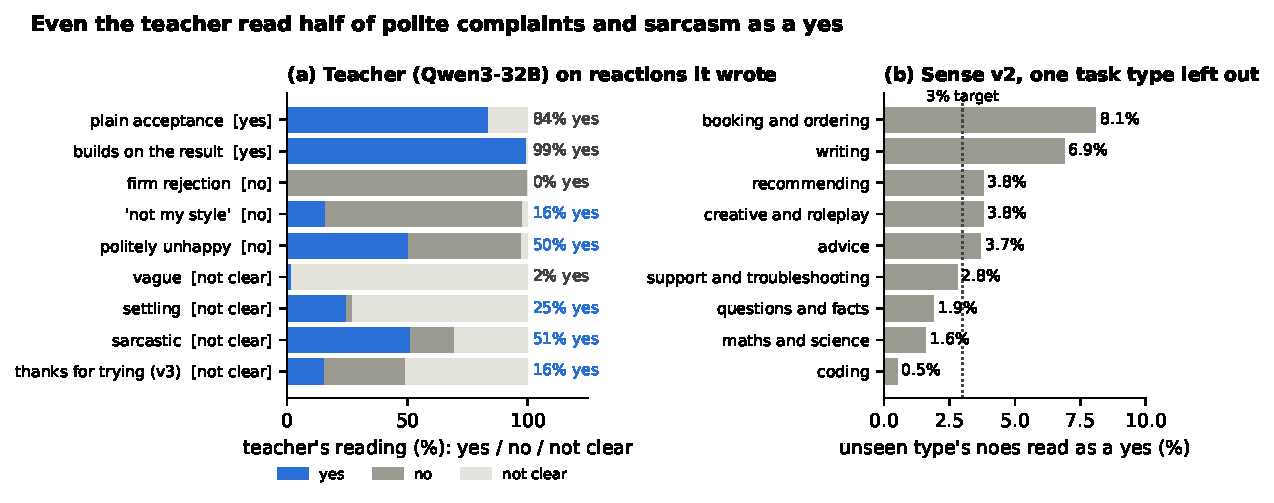
\includegraphics[width=1.0\linewidth]{figures/fig8_teacher_and_unseen_tasks}
\caption{(a) the v3 teacher's labels for the 6,506 reactions it wrote (sense3 build); (b) nine sense v2 builds, each trained without one task type and tested on it (sense2 leave-one-task-out runs)}
\label{fig:8}
\end{figure}

\emph{Sense v3.} It replaces v2's single question with two, because Experiment 3 showed where one question fails: warm thanks for the effort after a failure reads like approval (5.3). First, is the reaction a clear verdict on the result at all? Thanks for trying, sarcasm, hedging, settling, silence and moving on without a word are not. Only if it is: which score? The teacher answered both, under a revised guide, for 63,248 reactions: up to 2,000 for each pairing of task type and v2 answer, the eight written kinds again, and 1,778 new reactions of a ninth kind, warm thanks for the effort after a failure. It judged 41\% of them not clear. One LoRA learns both answers from 44,746 of them, the score weighted by how clear the teacher found the reaction. Its two thresholds, 0.80 for a clear verdict and 0.70 for the score, were chosen on 2,000 held-out reactions as the one that keeps false accepts, now also counting an unclear reaction read as a yes, at 3\% while keeping the most real yeses. On those reactions it kept 44\% of the teacher's yeses and agreed with the teacher's side on 95\% of the verdicts it gave. In use, a reaction must pass both gates before the creature learns from it (Fig.~\ref{fig:9}). The first gate changes how some common reactions are read (Table~\ref{tab:4}): moving on to the next request without a word was an 80, a half-weight yes, for v2, and thanks for trying could pass as approval; for v3, neither is a clear verdict.

\begin{figure}[htbp]
\centering
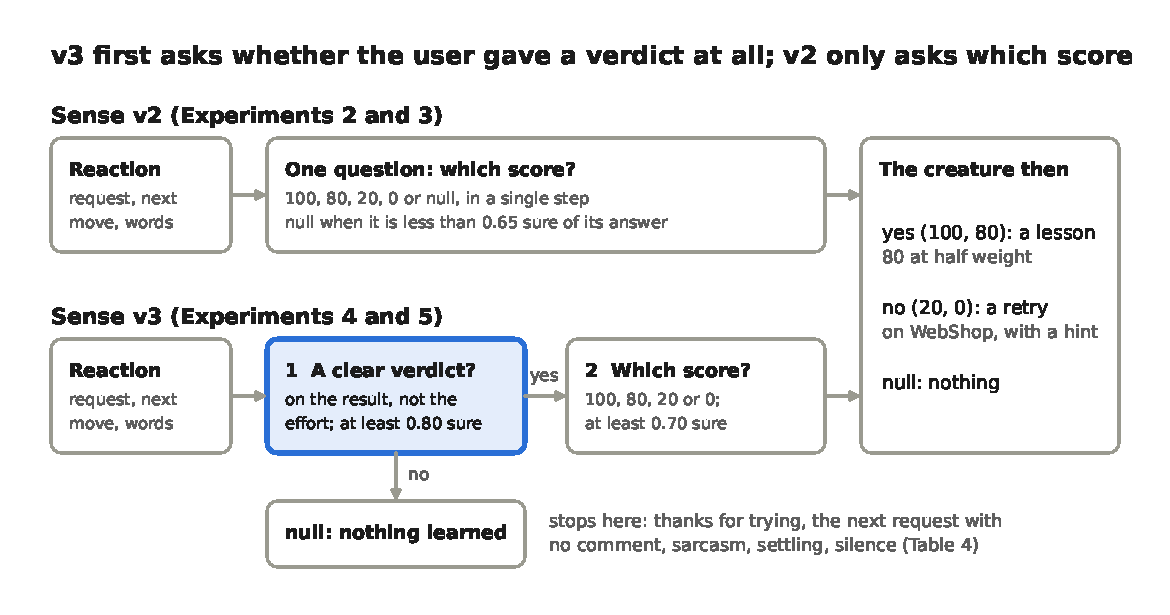
\includegraphics[width=1.0\linewidth]{figures/fig9_sense_decision}
\caption{How the two versions of the sense decide; thresholds from calibration (3.2), outcomes as in Table~\ref{tab:4}}
\label{fig:9}
\end{figure}

\begin{longtable}[]{@{}
  >{\raggedright\arraybackslash}p{(\linewidth - 8\tabcolsep) * \real{0.2857}}
  >{\raggedright\arraybackslash}p{(\linewidth - 8\tabcolsep) * \real{0.2222}}
  >{\raggedright\arraybackslash}p{(\linewidth - 8\tabcolsep) * \real{0.1429}}
  >{\raggedright\arraybackslash}p{(\linewidth - 8\tabcolsep) * \real{0.0635}}
  >{\raggedright\arraybackslash}p{(\linewidth - 8\tabcolsep) * \real{0.2857}}@{}}
\caption{How v2 and v3 read the same reactions, and what the creature does. Examples from the two labelling guides; v3 first asks whether the reaction is a clear verdict, and scores it only if it is.}\label{tab:4}\tabularnewline
\toprule\noalign{}
\begin{minipage}[b]{\linewidth}\raggedright
Reaction
\end{minipage} & \begin{minipage}[b]{\linewidth}\raggedright
v2
\end{minipage} & \begin{minipage}[b]{\linewidth}\raggedright
v3: clear verdict?
\end{minipage} & \begin{minipage}[b]{\linewidth}\raggedright
v3
\end{minipage} & \begin{minipage}[b]{\linewidth}\raggedright
What the creature does
\end{minipage} \\
\midrule\noalign{}
\endfirsthead
\toprule\noalign{}
\begin{minipage}[b]{\linewidth}\raggedright
Reaction
\end{minipage} & \begin{minipage}[b]{\linewidth}\raggedright
v2
\end{minipage} & \begin{minipage}[b]{\linewidth}\raggedright
v3: clear verdict?
\end{minipage} & \begin{minipage}[b]{\linewidth}\raggedright
v3
\end{minipage} & \begin{minipage}[b]{\linewidth}\raggedright
What the creature does
\end{minipage} \\
\midrule\noalign{}
\endhead
\bottomrule\noalign{}
\endlastfoot
``Perfect, exactly what I needed'' & 100 & yes & 100 & learns it as a lesson, full weight \\
``Ok, that works'' & 80 & yes & 80 & learns it as a lesson, half weight \\
``Great, now can you also\ldots{}'' (building on it) & 80 & yes & 80 & learns it as a lesson, half weight \\
the next request, with no comment & 80 & no & null & v2: learns at half weight; v3: nothing \\
``Thank you so much for trying! I'll look on my own'' & often a yes (Example 1, 5.3) & no & null & v2: often learns a failure; v3: nothing \\
``I guess that'll do''; ``hmm''; silence & null & no & null & nothing \\
``I said size 9'' & 20 & yes & 20 & retries, told to change only what the user asked for \\
``No, that's not what I asked''; repeats the request & 0 & yes & 0 & retries, told to start again and read the request carefully \\
\end{longtable}

\emph{Which sense, and what it has seen.} Experiments 2 and 3 use sense v2; Experiments 4 and 5 use sense v3, frozen in every life. Neither version trained on shopping or on our simulated users' words. But v3 is not blind to the WebShop user's failure: its ninth kind of reaction was added because Experiment 3 exposed it, and its test on recorded reactions (5.4, Fig.~\ref{fig:3}) uses that user's words. Section 6 tests it on a customer we did not design.

\section{Experimental setup}

We ran five experiments on two benchmarks, each with an \emph{oracle} condition as the upper bound and several seeds per condition (Table~\ref{tab:1}).

\textbf{Benchmarks.} WebShop \cite{yao2022webshop} (Experiments 1-4) is a simulated online shop with 1.18 million real products and 12,087 shopping requests written by crowd workers. The creature reads a request, searches, browses and buys; an attempt ends with a purchase or after 15 steps. The reward, 0 to 1, scores how well the bought product matches the request on its type, attributes, options and price \cite{yao2022webshop}. $\tau^2$-bench \cite{barres2026tau2} (Experiment 5), which extends $\tau$-bench \cite{yao2025taubench}, is a customer-service benchmark: the agent talks with a simulated customer and calls the domain's tools to change bookings, orders or phone plans under a written policy. Success is judged from the final state of the database. In telecom both sides act: the customer also uses tools on their own phone, as the agent directs \cite{barres2026tau2}. We used the train and test splits published in $\tau^2$-bench's repository and its airline, retail and telecom domains, with Gemini 3 Flash as the customer and as $\tau^2$-bench's graders in place of the published GPT models. Scores are therefore comparable to published ones, not identical.

\textbf{Simulated users.} We wrote WebShop's simulated user. In Experiments 1 and 2 it reacts plainly to the outcome: it stays silent 20\% of the time and otherwise says one fixed kind of sentence per outcome (no purchase, wrong kind of product, close but missing an option, perfect). From Experiment 3 on it reacts as people do: its behaviour is drawn from a mix tied to the outcome and to a persona (clear thanks, complaints, polite give-ups, vague replies, moving on without a word), and Gemini words each reaction (Table~\ref{tab:A2}; prompt in Appendix A). Because we designed this user, results that depend on it carry that design, and the sense's live test (5.4) uses its reactions. Two things limit the risk: the sense was never trained on shopping reactions, and Section 6 tests it against a simulated customer we did not design ($\tau^2$-bench's).

\textbf{Protocol.} The first 100 of WebShop's synthetic goals are held out from practice; the exam uses 50 of them, plus 13 written by people, every morning. With the \emph{oracle} as judge, an attempt with reward 0.5 or more becomes a lesson; we call an attempt below 0.5 a failure throughout. An attempt judged bad by any judge other than the \emph{oracle} gets one retry, with the user's comment and the creature's own lesson as a hint (Appendix A); a successful retry becomes a lesson (without the hint) and a preference pair (the retry over the failed attempt). $\tau^2$-bench has no retry: the customer cannot be asked to react twice.

\begin{longtable}[]{@{}
  >{\raggedright\arraybackslash}p{(\linewidth - 8\tabcolsep) * \real{0.1274}}
  >{\raggedright\arraybackslash}p{(\linewidth - 8\tabcolsep) * \real{0.2293}}
  >{\raggedright\arraybackslash}p{(\linewidth - 8\tabcolsep) * \real{0.1847}}
  >{\raggedright\arraybackslash}p{(\linewidth - 8\tabcolsep) * \real{0.2293}}
  >{\raggedright\arraybackslash}p{(\linewidth - 8\tabcolsep) * \real{0.2293}}@{}}
\caption{The experiments.}\label{tab:1}\tabularnewline
\toprule\noalign{}
\begin{minipage}[b]{\linewidth}\raggedright
\end{minipage} & \begin{minipage}[b]{\linewidth}\raggedright
Question
\end{minipage} & \begin{minipage}[b]{\linewidth}\raggedright
Benchmark, model
\end{minipage} & \begin{minipage}[b]{\linewidth}\raggedright
Judges
\end{minipage} & \begin{minipage}[b]{\linewidth}\raggedright
Seeds $\times$ days
\end{minipage} \\
\midrule\noalign{}
\endfirsthead
\toprule\noalign{}
\begin{minipage}[b]{\linewidth}\raggedright
\end{minipage} & \begin{minipage}[b]{\linewidth}\raggedright
Question
\end{minipage} & \begin{minipage}[b]{\linewidth}\raggedright
Benchmark, model
\end{minipage} & \begin{minipage}[b]{\linewidth}\raggedright
Judges
\end{minipage} & \begin{minipage}[b]{\linewidth}\raggedright
Seeds $\times$ days
\end{minipage} \\
\midrule\noalign{}
\endhead
\bottomrule\noalign{}
\endlastfoot
Experiment 1 & Who should decide what is learned? Does the decline pass with time, or depend on the adapter? & WebShop, 0.6B & \emph{oracle}, \emph{self}, \emph{both}, \emph{stated verdict}, \emph{none}; \emph{both} over a year; \emph{both} with four adapter designs & 5 $\times$ 14 (pilot 1 $\times$ 6); 5 $\times$ 365; 5 $\times$ 14 \\
Experiment 2 & Does a separate, frozen judge help? & WebShop, 0.6B & \emph{oracle}, \emph{both}, \emph{sense v2} & 5 $\times$ 14 \\
Experiment 3 & Does it survive realistic users? & WebShop, 0.6B, realistic user & \emph{oracle}, \emph{both}, \emph{sense v2}; then the same with lessons counted once & 5 $\times$ 14, twice \\
Experiment 4 & Does waiting for a clear verdict help? & WebShop, 0.6B, realistic user & \emph{oracle}, \emph{both}, \emph{sense v3} & 5 $\times$ 60 \\
Experiment 5 & What if the user cannot see the outcome? & $\tau^2$-bench, 0.6B and 1.7B & \emph{oracle}, \emph{sense v3} & 3 $\times$ 30 per size \\
\end{longtable}

\textbf{Measures.} The exam score over days, as the mean of seeds with the lowest and highest life; the number of lessons a day; the share of lessons whose attempt had truly succeeded; and, for the sense, its accuracy on a fixed set of recorded reactions. Statistics treat each life as one sample; two groups are compared with a Welch t-test and a Mann-Whitney U test, and the primary claims are Holm-corrected \cite{holm1979}. Appendix B lists every test, and src/stats.py in the repository recomputes them.

\textbf{Compute.} Lives ran on single NVIDIA L4 GPUs on Google Cloud, one or two lives per GPU. In all, 127 lives ran for about 1,300 hours and made about 490,000 attempts, practice and exams together. On WebShop a night's training took 1-4 minutes (median 2, the 0.6B \emph{oracle} life of Experiment 4). Building the two senses, teacher labels and student training, took about 7 GPU-hours.

\section{Results on WebShop}

On WebShop the judge decided each life. With the true outcome as judge, the creature rose from 13 to 62 within a week and held there; self-judging rose and then fell, \emph{sense v2} collapsed when it let polite give-ups in, and \emph{sense v3}, which waits for a clear verdict, came close to the \emph{oracle} for two weeks before fading. Across all lives, the share of failed attempts among the lessons decided the outcome (5.6).

This section follows one line: the problem (5.1), the idea (5.2), its first failure (5.3), the fix (5.4) and the fix's limit over time (5.5). Scores are the WebShop exam: the mean reward, 0 to 100, on 50 held-out tasks never learned from. Each number is the mean of 5 seeds with the lowest and highest life in brackets.

\subsection{Who should decide what the creature learns?}

Experiment 1 ran five lives that differed only in the judge, 5 seeds each for 14 days: the \emph{oracle} (the true reward), the user's \emph{stated verdict}, the creature's own reflection (\emph{self}), its reflection while hearing the user (\emph{both}), and no sleep at all (\emph{none}).

\begin{figure}[htbp]
\centering
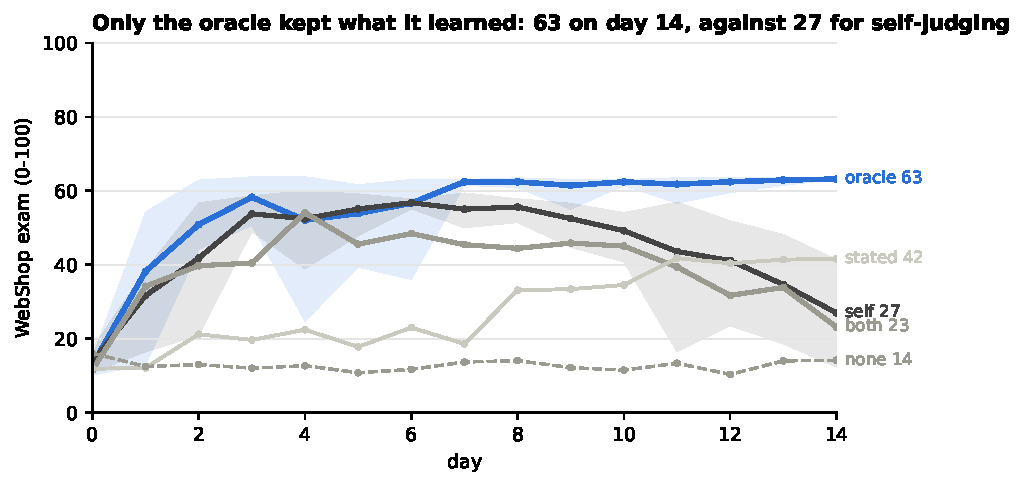
\includegraphics[width=1.0\linewidth]{figures/fig2_exp1_judges}
\caption{Experiment 1, 5 seeds per judge, daily exams; one self life crashed early and is left out}
\label{fig:2}
\end{figure}

On day 14 the \emph{oracle} averaged 63.2 $\pm$ 0.2 (mean $\pm$ standard deviation over seeds), \emph{self} 27.0 $\pm$ 11.9, \emph{both} 23.1 $\pm$ 17.0, \emph{stated verdict} 41.6 $\pm$ 23.1 and \emph{none} 14.2 $\pm$ 2.2. The \emph{stated verdict} learned from only 0-7 lessons per life, none of them a failure; three of its lives reached 54-61 and two stayed at 14-19. The \emph{oracle} beat \emph{self} and \emph{both} clearly (Welch t-test, p = 0.009 and 0.006); with 4-5 seeds, self-judging did not end reliably above no learning at all (p = 0.12).

Self-judging learned as fast as the \emph{oracle} at first and then lost most of it. By day 7 the \emph{self} and \emph{both} lives had reached 45-55; by day 14 every one of those nine lives had fallen below its own day-7 score, one to 0. The \emph{oracle} reached 62 by day 7 and stayed there. The \emph{stated verdict} rose slowly and unevenly (14-61 on day 14). One \emph{self} life crashed early and is left out. A 6-day pilot showed the same shape: the \emph{self} life rose from 13 to 34 by day 1 and fell to 9 by day 6.

\textbf{Does the decline pass with time?} We let the \emph{both} creature, the self-judge that also hears the user and the one that learned fastest early on, live for a year: 365 days, 5 seeds, beside one \emph{oracle} life. WebShop's practice tasks run out after about 227 days, so later days revisit old tasks.

\begin{figure}[htbp]
\centering
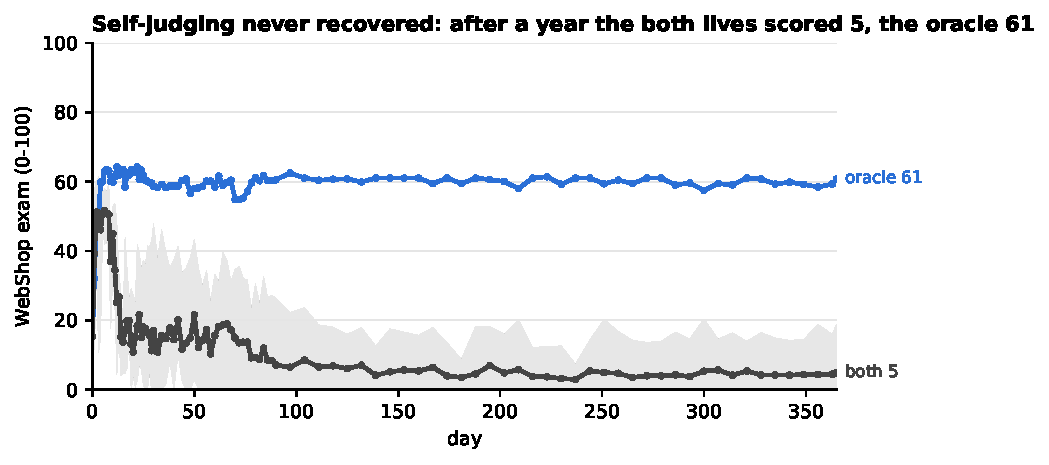
\includegraphics[width=1.0\linewidth]{figures/fig7_year_of_life}
\caption{Experiment 1, year of life: 5 both lives and 1 oracle life; exams daily to day 30, every 2 days to day 90, then weekly}
\label{fig:7}
\end{figure}

It never recovered. The \emph{both} lives peaked around day 6 (52, lives 42-58), were back at their starting level of 15 by day 14, and ended the year at 5 (0-19), three of the five at 0. The \emph{oracle} life rose from 15 to 64 by day 14 and stayed between 55 and 64 for the rest of the year (61 on day 365). These are separate lives from the 14-day \emph{both} condition above (23 on day 14, lives 0-46); the two ranges overlap. A first attempt at this run crashed when two nights ran out of GPU memory at once and was restarted from scratch.

\textbf{Is it the adapter?} If the adapter simply overwrote what it had learned, an adapter built to protect old learning might stop the decline. We gave the \emph{both} creature four designs, 5 seeds each for 14 days: one LoRA that keeps growing (as everywhere else), a LoRA whose learning rate halves every 4 days, a new rank-8 LoRA every 2 days with the older ones frozen, and the same with each new one smaller (rank 8 down to 1). All four peaked at 46-53 on day 7 and fell to 26-38 by day 14; the best of them still lost more than a quarter of its peak.

Neither time nor the adapter explains the decline. What the judge lets in does, and the rest of this section follows that thread.

\subsection{A separate, frozen judge: sense v2}

Experiment 2 gave the creature a judge it cannot change: the feedback sense (v2), a frozen Qwen3-0.6B with its own LoRA that reads the user's reaction to each attempt. It ran against the \emph{oracle} and \emph{both}, 5 seeds, 14 days, with the same user as Experiment 1.

{\def\LTcaptype{none} % do not increment counter
\begin{longtable}[]{@{}llll@{}}
\toprule\noalign{}
Judge & Day 0 & Day 7 & Day 14 \\
\midrule\noalign{}
\endhead
\bottomrule\noalign{}
\endlastfoot
\emph{oracle} & 11 & 62 (61-63) & 62 (61-63) \\
\emph{sense v2} & 13 & 19 (7-43) & 40 (6-59) \\
\emph{both} & 13 & 47 (36-57) & 16 (3-32) \\
\end{longtable}
}

\emph{Sense v2} learned more slowly but did not fall back. It also learned from very little: 0-7 lessons per life in 14 days, against 247-274 for the \emph{oracle}. By day 14, four of its five lives stood at 34-59 and were still rising, while every \emph{both} life had fallen from its day-7 peak. On day 14 \emph{sense v2} (39.7 $\pm$ 21.3) was ahead of \emph{both} (16.1 $\pm$ 11.1) and behind the \emph{oracle} (62.0 $\pm$ 1.0). With 5 seeds and one \emph{sense v2} life at 6, the t-test finds neither gap significant (p = 0.07 and 0.08); a rank test, less swayed by that one life, puts the gap to the \emph{oracle} at p = 0.01 (Appendix B). Sense v2's own accuracy stayed fixed, as intended: on 300 recorded reactions it read 82.6\% correctly on day 0 and 82.8\% on day 14. A variant that read the sense through the creature's learning brain was planned, but its lives scored 0 from day 0 because of a setup fault and were stopped; it is not reported.

\subsection{Realistic users break sense v2}

Experiment 3 replaced the user with one that reacts as people do. Its behaviour is drawn from a mix tied to the outcome and a persona, and worded by Gemini: clear thanks, complaints, but also polite give-ups, vague replies and moving on without a word. \emph{Oracle}, \emph{both} and \emph{sense v2}, 5 seeds, 14 days.

The \emph{sense v2} lives split in two. Two reached 55 and 57 by day 14, close to the \emph{oracle}'s 62. The other three fell to 0-3 on day 1 and never recovered. Each had learned on night 1 from one to three polite give-ups that sense v2 had read as success (Example 1 below); 96-100\% of everything those three lives learned were failed attempts. The \emph{both} lives rose to 48 by day 3 and fell to 15 (2-36). On day 14 the \emph{sense v2} lives averaged 22.5 $\pm$ 30.8 against the \emph{oracle}'s 62.0 $\pm$ 1.1 (Welch t-test p = 0.045, Mann-Whitney p = 0.01); the spread is the split itself.

\textbf{Example 1: a give-up sense v2 took for success (Experiment 3, night 1).} The shopper asked for men's loafers in size 6.5 under \$60. The creature bought nothing (reward 0). The user ended:

\begin{quote}
``That's perfectly fine, thank you so much for trying to help me! I think I'll just leave it for now and head out.''
\end{quote}

Sense v2 scored this reaction 100, the top score, with confidence 0.92, and the attempt became a lesson. All five practice attempts that became bad lessons on night 1 in the three collapsed lives look like this: warm thanks for the effort, then the user leaves.

Changing sleep did not remove the cause. When each lesson counted once, however many steps it took, and the creature slept only after 5 lessons, fewer lives collapsed, but 2 of 5 still ended at 0-3. The fault was in the judge, not the sleep.

\subsection{Waiting for a clear verdict: sense v3}

Experiment 4 used sense v3 (Section 3), our fullest attempt at discernment. It first asks whether the reaction is a clear verdict on the result; thanks for the effort, sarcasm, hedging, silence or moving on count as no verdict, and nothing is learned from them. Only a clear verdict is then scored. Same user and conditions as Experiment 3.

On 2,622 recorded reactions from Experiment 3, sense v3 read 1.2\% of reactions that were neither praise nor acceptance as a yes, against 5.0\% for v2, and read 1.0\% of give-ups and polite complaints as success, against 15.8\% (Fig.~\ref{fig:3}; Fisher exact test, p \textless{} 0.001). The price was a stricter reading of real approval: it took 59\% of plain acceptances as a yes, against 70\% for v2. In the lives, four of five \emph{sense v3} lives stood at 53-60 on day 14, against the \emph{oracle}'s 63 (62-63). Averaged over all five lives \emph{sense v3} (45.1 $\pm$ 25.3) was not reliably below the \emph{oracle} by a t-test (62.8 $\pm$ 0.6; p = 0.19), because the one collapsed life dominates the spread; by a rank test it was (p = 0.01), since every \emph{sense v3} life scored below every \emph{oracle} life. The fifth fell to 0 after learning from a single give-up on night 1. The \emph{both} lives peaked at 53 on day 7 and fell to 19 by day 14, as before.

\begin{figure}[htbp]
\centering
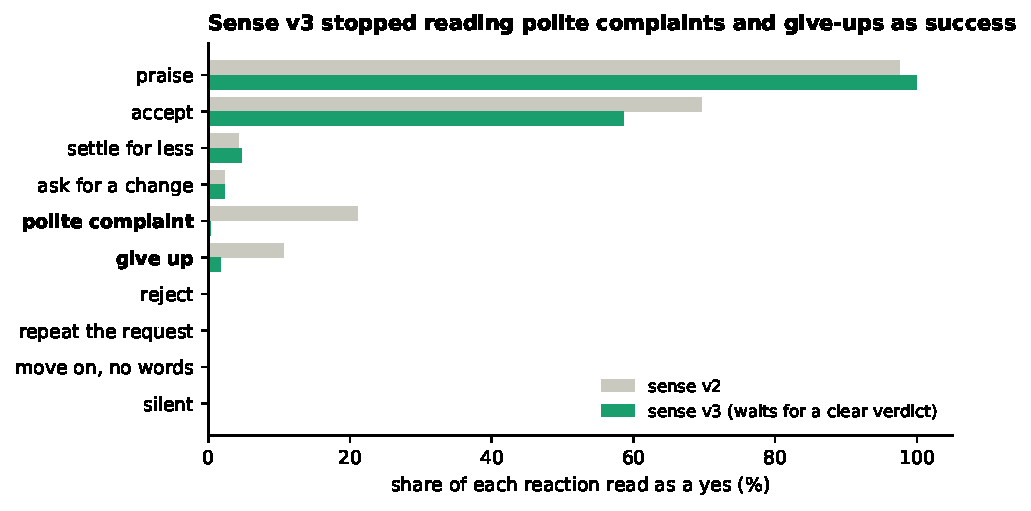
\includegraphics[width=1.0\linewidth]{figures/fig3_sense_v2_v3}
\caption{Sense live test: up to 300 recorded reactions per behaviour from the Experiment 3 lives (2,622 in all), read by both versions of the sense}
\label{fig:3}
\end{figure}

\subsection{Clean but scarce lessons fade: sense v3 over 60 days}

Every life of Experiment 4 was extended to 60 days.

\begin{figure}[htbp]
\centering
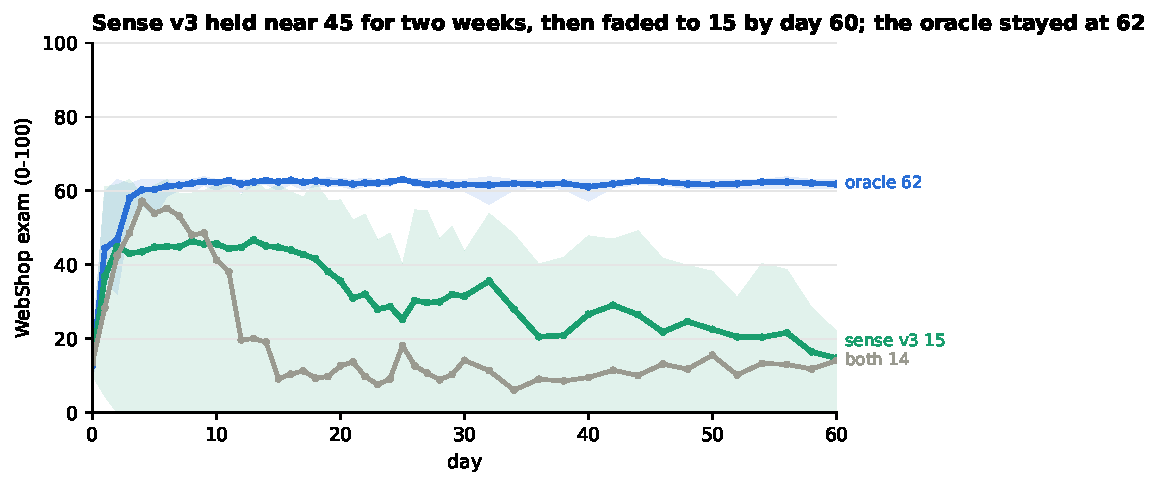
\includegraphics[width=1.0\linewidth]{figures/fig4_sense_v3_60_days}
\caption{Experiment 4, 5 seeds per judge, 60 days; exams daily to day 30, then every 2 days}
\label{fig:4}
\end{figure}

Life by life, the four \emph{sense v3} lives that did not collapse stood at 53-60 on day 14, 36-44 on day 30 and 9-22 on day 60; the fifth stayed at 0 throughout. On day 60 the \emph{oracle} (61.8 $\pm$ 0.9) was far above \emph{sense v3} (14.7 $\pm$ 9.7; Welch t-test p \textless{} 0.001).

The four \emph{sense v3} lives declined steadily after day 14, although what they learned stayed clean. They took in about 2 lessons a day (1.6-2.4), against the \emph{oracle}'s 20-21, and learned from only 10-13\% of their own good attempts, because a clear yes was rare. Over the 60 days only 2-10\% of their lessons were failed attempts. The collapsed life stayed at 0 for all 60 days, replaying its bad lessons (Fig.~\ref{fig:4}). Why they faded is open. Scarcity alone is not an obvious answer, since in Experiment 2 lives with even fewer lessons kept rising to day 14; an \emph{oracle} limited to 2 lessons a day would settle it.

\subsection{What every life has in common}

Across the WebShop experiments (1-4, including the adapter designs of 5.1), what decided a life was the share of its lessons that were failed attempts, not the number of lessons or the kind of judge.

\begin{figure}[htbp]
\centering
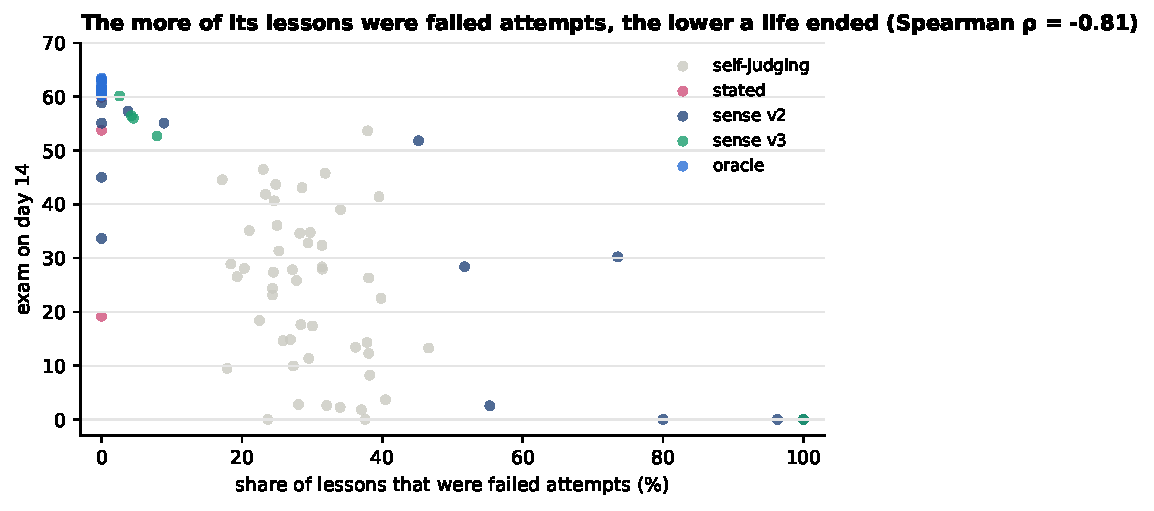
\includegraphics[width=1.0\linewidth]{figures/fig6_failed_lessons}
\caption{All 14-day WebShop lives in Experiments 1-4, including the adapter designs of 5.1, that learned at least once (97 of 104); lessons counted to day 14; Exp 3b = the sleep variant of Experiment 3}
\label{fig:6}
\end{figure}

Across 97 lives, the share of failed attempts among a life's lessons in its first 14 days predicted its day-14 exam closely (Spearman $\rho$ = -0.81, p \textless{} 0.001). The \emph{oracle} lives, all at 0\% failures and about 63, do not drive this alone: among the 72 lives not judged by the \emph{oracle}, $\rho$ = -0.61 (p \textless{} 0.001). Every \emph{oracle} life learned only from successes and ended at 60-63. Self-judging lives let in 17-47\% failures and ended anywhere from 0 to 54. The sense lives, v2 and v3 together, split cleanly: the ten that let in under 10\% failures ended at 34-60; the nine that let in 45\% or more ended at 0-52, six of them at 0-3.

The number of lessons mattered less than we expected. In Experiment 2 the \emph{sense v2} lives learned from only 0-7 lessons in 14 days and still reached 34-59; in Experiment 1, the \emph{stated verdict} learned from 0-7, none of them failures, and reached up to 61. A few correct lessons are enough to teach the shop's basic routine, and a few wrong ones are enough to undo it.

This explains why a single bad night can end a sense life. A sense life learned from only 0-6 lessons on night 1, so one failed attempt could be most of its first night's training. Of the 20 sense lives in Experiments 2-4 (v2 in Experiments 2 and 3, v3 in Experiment 4), seven learned from a failed attempt on night 1, and six of those seven ended at 0-3 (Fisher exact test, p \textless{} 0.001). Of the thirteen without one, none ended below 28, except one that never learned anything at all (6).

\section{Results on $\tau^2$-bench}

On $\tau^2$-bench, learning from customer reactions taught the agent to fail, and even learning from the true outcome did not raise its overall score.

Experiment 5 put the creature in $\tau^2$-bench's customer-service role, with Gemini 3 Flash playing the customer. Qwen3 0.6B and 1.7B each lived 30 days, 3 seeds per condition. Each day the agent served 30 customers from the airline and retail training tasks; each night it learned from the conversations judged good, either by the \emph{oracle} ($\tau^2$-bench's own check of the final database) or by the frozen \emph{sense v3} reading how the customer ended the conversation. Every 3 days it sat an exam on the official test tasks, never learned from: airline (20), retail (40) and telecom (40), a domain it never practised.

\subsection{Without learning}

The plain models solved a few tasks in each domain: 0.6B 5\% of retail, 35\% of airline and 33\% of telecom; 1.7B 18\%, 25\% and 35\%; 4B, for reference, 16\% (on the 32 retail tasks that ran without error), 20\% and 30\%. Retail separates the sizes best, because every success needs 4-16 correct tool calls. Some airline successes are tasks where the right answer is to refuse, and many telecom successes need one agent action while the customer fixes their own phone.

\subsection{The customer cannot judge}

Before any learning, we let sense v3 read how the 292 baseline conversations ended and compared its verdict with the true outcome. 20 of its 34 yeses came after failed tasks. The sense read the customers correctly: they ended with clear, sincere thanks, for example ``Alright, that's great, thanks a lot.'' But the customer cannot see the database, so it often thanks the agent after a wrong payment method, a broken rule or a missed detail. Retail separated well (a yes after 50\% of done tasks, 6\% of failed ones); airline did not (6\% against 30\%).

\subsection{Learning from reactions collapses}

In the lives, it was worse. Only 20\% of the conversations sense v3 accepted had in fact succeeded (47 of 232 for 1.7B, 42 of 212 for 0.6B), and sense v3 missed most real successes, learning from 10-20\% of them. All three 1.7B \emph{sense v3} lives ended near zero on day 30: airline 25\% to 2\%, retail 11\% to 3\%, telecom 33\% to 8\%; over all exam tasks they fell from 23\% to 4\% (paired t-test over the 3 lives, p = 0.03). With 3 lives per condition and the \emph{oracle} lives also falling on two domains, the day-30 gap to the 1.7B \emph{oracle} (13\%) is not significant (p = 0.12). One stopped completing tasks within nine days: its practice success fell from 17\% in days 1-5 to under 1\% in days 21-25, while its conversations grew longer, from about 15 to 22 agent turns. The 0.6B \emph{sense v3} lives survived because they learned little, about 2 conversations a day; their airline and retail scores did not move, and telecom fell in one of the three.

\textbf{Example 2: a thanked failure (Experiment 5, 1.7B \emph{sense v3} life, day 2).} A customer asked to cancel all their upcoming flights. The agent did not complete the task (reward 0). The customer ended: ``C'est parfait. Merci pour votre aide. That is all I needed.'' Sense v3 scored it 100 with confidence 0.99, and it became a lesson.

\subsection{Correct lessons, lopsided}

The \emph{oracle}'s lessons were all correct, yet they shifted skill rather than adding it. About three quarters came from airline (72\% for 1.7B, 77\% for 0.6B), where the small models succeed more often, although retail has more than twice as many training tasks. The 1.7B \emph{oracle} lives rose on airline from 28\% to 35\% (all three ended at 35\%), fell on retail from 11\% to 6\%, and fell on telecom from 32\% to 10\%. Telecom fell in 4 of the 6 \emph{oracle} lives, three of them to 0-2\%. Forgetting of this kind could only show here: on WebShop every task is the same kind of task.

\begin{figure}[htbp]
\centering
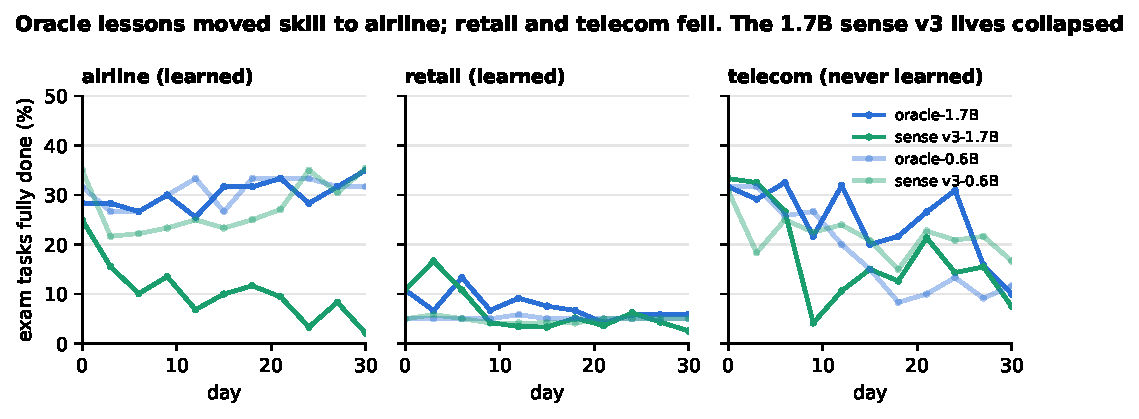
\includegraphics[width=1.0\linewidth]{figures/fig5_tau2_domains}
\caption{Experiment 5, 3 seeds per condition; exams on day 0 and every 3 days; broken exam conversations left out}
\label{fig:5}
\end{figure}

{\def\LTcaptype{none} % do not increment counter
\begin{longtable}[]{@{}
  >{\raggedright\arraybackslash}p{(\linewidth - 10\tabcolsep) * \real{0.1565}}
  >{\raggedright\arraybackslash}p{(\linewidth - 10\tabcolsep) * \real{0.1565}}
  >{\raggedright\arraybackslash}p{(\linewidth - 10\tabcolsep) * \real{0.1565}}
  >{\raggedright\arraybackslash}p{(\linewidth - 10\tabcolsep) * \real{0.2000}}
  >{\raggedright\arraybackslash}p{(\linewidth - 10\tabcolsep) * \real{0.1217}}
  >{\raggedright\arraybackslash}p{(\linewidth - 10\tabcolsep) * \real{0.2087}}@{}}
\toprule\noalign{}
\begin{minipage}[b]{\linewidth}\raggedright
Condition
\end{minipage} & \begin{minipage}[b]{\linewidth}\raggedright
Airline (learned)
\end{minipage} & \begin{minipage}[b]{\linewidth}\raggedright
Retail (learned)
\end{minipage} & \begin{minipage}[b]{\linewidth}\raggedright
Telecom (never learned)
\end{minipage} & \begin{minipage}[b]{\linewidth}\raggedright
Lessons a day
\end{minipage} & \begin{minipage}[b]{\linewidth}\raggedright
Lessons truly successful
\end{minipage} \\
\midrule\noalign{}
\endhead
\bottomrule\noalign{}
\endlastfoot
\emph{oracle} 1.7B & 28 $\rightarrow$ 35 & 11 $\rightarrow$ 6 & 32 $\rightarrow$ 10 & 5.3 & 100\% \\
\emph{sense v3}, 1.7B & 25 $\rightarrow$ 2 & 11 $\rightarrow$ 3 & 33 $\rightarrow$ 8 & 2.6 & 20\% \\
\emph{oracle} 0.6B & 32 $\rightarrow$ 32 & 5 $\rightarrow$ 5 & 32 $\rightarrow$ 12 & 5.2 & 100\% \\
\emph{sense v3}, 0.6B & 35 $\rightarrow$ 35 & 5 $\rightarrow$ 5 & 31 $\rightarrow$ 17 & 2.4 & 20\% \\
\end{longtable}
}

Share of exam tasks fully done, day 0 $\rightarrow$ day 30, mean of 3 seeds. Exams are small: one airline task is 5 points, one retail or telecom task 2.5, so moves under about 10 points are within noise. Exam conversations that broke, for example a loop past the length limit, are left out; counting them as failures would lower the collapsed lives further. The 0.6B never moved on retail: every exam of every 0.6B life scored exactly 5\%, the same two tasks each time.

\section{Discussion}

Three conditions decide whether learning from users works: the judge keeps failed attempts out of the lessons, the user can see the outcome so that this is possible, and lessons cover the skills evenly.

\begin{itemize}
\tightlist
\item
  \textbf{Precision matters more than volume.} A handful of correct lessons was enough to improve (5.6), while one failed attempt on night 1 could end a life. A judge should refuse to learn when in doubt. Why clean but sparse lessons still faded after two weeks (5.5) is open.
\item
  \textbf{Discernment is bounded by what the user can see.} The sense read customers correctly; the customers were wrong. No amount of discernment in reading a reaction can recover what the user did not know.
\item
  \textbf{Replay follows success.} Lessons come from what the model already does well, so replay narrows its skills; balancing by domain or task type is the obvious fix.
\item
  \textbf{Practical advice:} ask users for a verdict only when they can check the result; mix in verified outcomes where available; balance replay across skills.
\item
  \textbf{To write: future work.} A fix for forgetting (replay balanced by domain or task type, tested on $\tau^2$-bench); an explanation of the late fade (an \emph{oracle} limited to about 2 lessons a day); a test of the sense on real users' reactions; larger models.
\end{itemize}

\section{Limitations}

\begin{itemize}
\tightlist
\item
  Small models only (0.6B and 1.7B); larger models may judge themselves better.
\item
  Simulated users throughout (our own on WebShop, Gemini on $\tau^2$-bench); real users may give more or fewer clear verdicts.
\item
  3-5 seeds and small exams (one $\tau^2$-bench airline task is 5 points).
\item
  $\tau^2$-bench run with Gemini as customer and grader, not the published GPT simulator; scores are comparable, not identical.
\item
  No fix for forgetting or for the late fade was tested. The judges are simplified stand-ins for published methods, not their original implementations. We designed the WebShop user, and the sense's live test uses its reactions.
\end{itemize}

\section{Conclusion}

Nightly self-training lets a small model improve on the job only while failed attempts stay out of its lessons. Knowing the true outcome is the surest way to keep them out, though on its own it did not prevent forgetting on $\tau^2$-bench. Discernment, reading the user's reaction for a clear and informed verdict, can stand in for that judge for a while, but only if the user can see the result. Where the user cannot, learning from users teaches failure.


\bibliographystyle{unsrtnat}
\bibliography{references}

\appendix
% Appendix tables and figures are numbered by appendix: A1, A2, ..., B1.
\counterwithin{table}{section}\counterwithin{figure}{section}
\renewcommand{\thetable}{\Alph{section}\arabic{table}}\renewcommand{\thefigure}{\Alph{section}\arabic{figure}}
\section{Settings}

\begin{longtable}[]{@{}
  >{\raggedright\arraybackslash}p{(\linewidth - 2\tabcolsep) * \real{0.5000}}
  >{\raggedright\arraybackslash}p{(\linewidth - 2\tabcolsep) * \real{0.5000}}@{}}
\caption{Settings used in every experiment unless noted.}\label{tab:A1}\tabularnewline
\toprule\noalign{}
\begin{minipage}[b]{\linewidth}\raggedright
Part
\end{minipage} & \begin{minipage}[b]{\linewidth}\raggedright
Setting
\end{minipage} \\
\midrule\noalign{}
\endfirsthead
\toprule\noalign{}
\begin{minipage}[b]{\linewidth}\raggedright
Part
\end{minipage} & \begin{minipage}[b]{\linewidth}\raggedright
Setting
\end{minipage} \\
\midrule\noalign{}
\endhead
\bottomrule\noalign{}
\endlastfoot
Creature & Qwen3-0.6B (WebShop); Qwen3-0.6B and 1.7B ($\tau^2$-bench); thinking off; vLLM \\
Practice & 30 tasks a day; temperature 0.7 (agent and $\tau^2$-bench customer) \\
Exams & temperature 0; WebShop 50 + 13 tasks daily; $\tau^2$-bench 20 + 40 + 40 tasks every 3 days \\
WebShop episode & at most 15 steps; last 2 pages kept in full; at most 25 clickable options shown \\
Learning adapter & LoRA rank 8, scale 20, top 8 layers, q/k/v/o and feed-forward projections, no dropout \\
Night & AdamW, learning rate 1e-4, 2 epochs, 10-40 steps, batch 4 ($\tau^2$-bench: 1), sequence 2,048 tokens ($\tau^2$-bench: 10,240) \\
Objective & SFT on the agent's replies, plus DPO ($\beta$ = 0.1) on preference pairs from corrected retries; reference = that morning's model \\
Replay & the 150 most recent lessons and pairs \\
Lesson weight & each step a lesson of its own (Experiments 1-3); spread across its steps (Experiment 3 variant, 4, 5) \\
\emph{Oracle} & reward 0.5 or more (WebShop); reward 1 ($\tau^2$-bench) \\
Sense & Qwen3-0.6B + LoRA rank 16, alpha 32, all attention and MLP projections; teacher Qwen3-32B (AWQ); one epoch, learning rate 1e-4, batch 16, KL to the teacher's probabilities, false accepts at most 3\% on 2,000 held-out reactions; v2: temperature 1.0, threshold 0.65, 47,800 training reactions; v3: thresholds 0.80 (clear verdict) and 0.70 (score), temperatures 1.0 and 1.05, 44,746 training reactions; a score of 80 counts at half weight \\
\end{longtable}

\begin{longtable}[]{@{}
  >{\raggedright\arraybackslash}p{(\linewidth - 2\tabcolsep) * \real{0.5000}}
  >{\raggedright\arraybackslash}p{(\linewidth - 2\tabcolsep) * \real{0.5000}}@{}}
\caption{The realistic user (Experiments 3 and 4). The outcome band sets the chance of each behaviour; a persona drawn at random (terse, chatty, picky, polite, easygoing, blunt) then scales it; Gemini 3 Flash words the reaction.}\label{tab:A2}\tabularnewline
\toprule\noalign{}
\begin{minipage}[b]{\linewidth}\raggedright
Outcome
\end{minipage} & \begin{minipage}[b]{\linewidth}\raggedright
Behaviour mix
\end{minipage} \\
\midrule\noalign{}
\endfirsthead
\toprule\noalign{}
\begin{minipage}[b]{\linewidth}\raggedright
Outcome
\end{minipage} & \begin{minipage}[b]{\linewidth}\raggedright
Behaviour mix
\end{minipage} \\
\midrule\noalign{}
\endhead
\bottomrule\noalign{}
\endlastfoot
nothing bought & give up 50\%, repeat the request 30\%, silent 20\% \\
wrong product & reject 50\%, repeat 20\%, give up 10\%, silent 20\% \\
partly right & ask for a change 40\%, settle 15\%, reject 10\%, accept 10\%, polite complaint 5\%, silent 20\% \\
mostly right (reward 0.75 or more) & accept 30\%, move on 20\%, ask for a change 20\%, settle 5\%, polite complaint 5\%, silent 20\% \\
exactly right & praise 40\%, accept 20\%, move on 20\%, silent 20\% \\
\end{longtable}

\begin{longtable}[]{@{}
  >{\raggedright\arraybackslash}p{(\linewidth - 4\tabcolsep) * \real{0.3333}}
  >{\raggedright\arraybackslash}p{(\linewidth - 4\tabcolsep) * \real{0.3333}}
  >{\raggedright\arraybackslash}p{(\linewidth - 4\tabcolsep) * \real{0.3333}}@{}}
\caption{What the sense learned from. Reactions the teacher labelled; training used a balanced sample of them (47,800 for v2, 44,746 for v3).}\label{tab:A3}\tabularnewline
\toprule\noalign{}
\begin{minipage}[b]{\linewidth}\raggedright
Source
\end{minipage} & \begin{minipage}[b]{\linewidth}\raggedright
Reactions
\end{minipage} & \begin{minipage}[b]{\linewidth}\raggedright
What they are
\end{minipage} \\
\midrule\noalign{}
\endfirsthead
\toprule\noalign{}
\begin{minipage}[b]{\linewidth}\raggedright
Source
\end{minipage} & \begin{minipage}[b]{\linewidth}\raggedright
Reactions
\end{minipage} & \begin{minipage}[b]{\linewidth}\raggedright
What they are
\end{minipage} \\
\midrule\noalign{}
\endhead
\bottomrule\noalign{}
\endlastfoot
WildFB \cite{peng2026wildreward} & 30,000 & WildChat users' follow-up turns, rated for satisfaction (MIT) \\
WildFeedback \cite{shi2026wildfeedback} & 30,000 & WildChat conversations annotated as satisfied or dissatisfied (ODC-BY) \\
Taskmaster 1-3 \cite{byrne2019taskmaster} & 20,000 & task dialogues: ordering, booking, tickets (CC BY 4.0) \\
MultiWOZ 2.2 \cite{zang2020multiwoz} & 15,000 & travel-booking dialogues (MIT) \\
ReDial \cite{li2018redial} & 15,000 & movie-recommendation dialogues (CC BY 4.0) \\
CCPE-M \cite{radlinski2019ccpe} & 906 & dialogues that draw out movie preferences (CC BY 4.0) \\
Written by the teacher & 4,728 & eight hard kinds $\times$ ten task types $\times$ six personas (v2 and v3) \\
Written by the teacher & 1,778 & warm thanks for the effort after a failure (v3 only) \\
\end{longtable}

\textbf{Prompts.} The exact text each model received; words in braces are filled in for each attempt. The code is in the repository (lab/agent.py, lab/creature.py, lab/user\_llm.py, lab/sense/\_\_init\_\_.py).

\emph{Agent, WebShop.} The system prompt; each turn the model also sees the current page, its clickable options and its earlier steps. On $\tau^2$-bench the agent used $\tau^2$-bench's own agent prompt and domain policy, unchanged.

\begin{verbatim}
You are a personal assistant for one user. You talk with them and can look things up.

Each turn, reply with JSON only:
{"thought": "<brief reasoning>", "action": "<one of: search, click>", "input": "<text>"}

Tools:
- "search": search the shop. Input: keywords.
- "click": click a product, option or button. Input: its exact text from 'Clickable'. Clicking 'Buy Now' ends the task.
The task ends when the environment says so.
\end{verbatim}

\emph{Reflection, for self and both.} The same model and system prompt for both judges:

\begin{verbatim}
You review your own past attempt at a shopping task, honestly.
Reply with JSON only: {"verdict": "good" or "bad", "lesson": "<one short sentence for next time>"}
"good" means the purchase matches the request. Say "bad" if anything clearly does not match.
\end{verbatim}

followed by this message. Only \emph{both} gets the user's words; \emph{self} gets ``The user said nothing.'', and \emph{both} gets ``(no comment; they moved on to their next request)'' when the user moved on without a word.

\begin{verbatim}
Task: {request}

What you did:
{the first 8 steps, one per line}

Result: {what was bought, or "nothing was bought"}
The user said: "{the user's words}"

Was your attempt good?
\end{verbatim}

\emph{Retry hint, WebShop.} Added below the first page of the retried task, and removed again before the retry becomes a lesson. The lesson is the reflection's for \emph{self} and \emph{both}; for the sense it is ``the user wants an adjustment; change only what they asked for'' after a 20 and ``the attempt was wrong; start again and read the request carefully'' after a 0; otherwise ``try again more carefully''.

\begin{verbatim}
Your last attempt at this task did not go well. The user said: "{the user's words}". Your lesson: {lesson}
\end{verbatim}

\emph{Feedback sense v2.} One call; the answer is the first token of 100, 80, 20, 0 or null.

\begin{verbatim}
You read how a user reacted to an AI assistant and score the assistant's attempt. Answer with one of: 100 (exactly right), 80 (acceptable), 20 (needs adjusting), 0 (wrong), null (unclear).
\end{verbatim}

\begin{verbatim}
Request: {request}
The user's next move: {replied | new request | asked to adjust | repeated the request | left the session | said nothing}
What the user said: {the user's words, or "(nothing)"}
Score:
\end{verbatim}

\emph{Feedback sense v3.} Two calls with the same message, ending ``Clear verdict:'' for the first question and ``Score:'' for the second. On $\tau^2$-bench the request is the customer's first message, the words their last one, and the next move ``left the session'' if the customer ended the conversation, else ``replied''. The teacher's labelling guides, about 80 lines each, are in the repository (lab/sense/guide.md for v2, lab/sense/guide3.md for v3).

\begin{verbatim}
You read how a user reacted to an AI assistant. Is the reaction a clear verdict on the assistant's result? Thanking the effort rather than the result, sarcasm, hedging, settling, silence, moving on without a word, or anything ambiguous is not clear. Answer yes or no.
\end{verbatim}

\begin{verbatim}
You read how a user reacted to an AI assistant; the reaction is a clear verdict on the result. Score the assistant's attempt: 100 (exactly right), 80 (acceptable, or building on it), 20 (one part missed what was asked), 0 (wrong).
\end{verbatim}

\emph{Realistic user, Experiments 3 and 4 (Gemini 3 Flash).} One call per reaction, after the behaviour and persona are drawn (Table~\ref{tab:A2}). Silence and moving on without a word need no call.

\begin{verbatim}
You are a shopper who asked an AI assistant to buy something for you.
Your request: {request}
What it bought: {title, options and price, or "nothing"}
Your personality: {style of the drawn persona}.
What you do now: {instruction for the drawn behaviour}
Write only your next message to the assistant, in your own words, one or two short sentences. Reply as JSON: {"said": "..."}
\end{verbatim}

\begin{longtable}[]{@{}
  >{\raggedright\arraybackslash}p{(\linewidth - 2\tabcolsep) * \real{0.5000}}
  >{\raggedright\arraybackslash}p{(\linewidth - 2\tabcolsep) * \real{0.5000}}@{}}
\caption{The realistic user's instruction for each behaviour (``What you do now''). Personas: terse (very short, few words, no pleasantries); chatty (friendly and talkative, a couple of sentences); picky (precise and demanding); polite (very polite, softens complaints); easygoing (relaxed and easily satisfied); blunt (blunt, casual, may use slang).}\label{tab:A4}\tabularnewline
\toprule\noalign{}
\begin{minipage}[b]{\linewidth}\raggedright
Behaviour
\end{minipage} & \begin{minipage}[b]{\linewidth}\raggedright
Instruction
\end{minipage} \\
\midrule\noalign{}
\endfirsthead
\toprule\noalign{}
\begin{minipage}[b]{\linewidth}\raggedright
Behaviour
\end{minipage} & \begin{minipage}[b]{\linewidth}\raggedright
Instruction
\end{minipage} \\
\midrule\noalign{}
\endhead
\bottomrule\noalign{}
\endlastfoot
praise & You are clearly happy: praise it or thank them warmly. \\
accept & You accept it without fuss, e.g.~a short `ok, thanks'. Do not praise it and do not complain. \\
ask for a change & Point out the one thing that missed what you asked for (\{the missed detail\}). Say it as something you had asked for (e.g.~`I wanted it in\ldots{}', `I said\ldots{}'), not as a new wish. \\
reject & Reject it: it is not what you asked for, or not your style. Do not ask for a small tweak. \\
repeat the request & Ask for the same thing again in your own words, as if the purchase did not happen: \{the request\} \\
polite complaint & Say thanks, but then ask for the same thing again in other words: \{the request\} \\
give up & Give up on it, in a few words, as you leave. \\
settle & Reluctantly settle for it in a flat, lukewarm way that does not say whether it is good. \\
\end{longtable}

\section{Statistics}

Every test in the paper, recomputed from the experiment databases by paper/stats.py in the repository. Each life (one seed) is one sample. Two-group comparisons are reported as a Welch t-test and a Mann-Whitney U test, because sense lives either stay near the \emph{oracle} or collapse, so the data are not bell-shaped. The six primary claims (marked $\star$) are Holm-corrected as one family; the others are supporting.

\begin{longtable}[]{@{}
  >{\raggedright\arraybackslash}p{(\linewidth - 6\tabcolsep) * \real{0.2500}}
  >{\raggedright\arraybackslash}p{(\linewidth - 6\tabcolsep) * \real{0.2500}}
  >{\raggedright\arraybackslash}p{(\linewidth - 6\tabcolsep) * \real{0.2500}}
  >{\raggedright\arraybackslash}p{(\linewidth - 6\tabcolsep) * \real{0.2500}}@{}}
\caption{Statistical tests.}\label{tab:B1}\tabularnewline
\toprule\noalign{}
\begin{minipage}[b]{\linewidth}\raggedright
Claim
\end{minipage} & \begin{minipage}[b]{\linewidth}\raggedright
Groups (mean $\pm$ SD, lives)
\end{minipage} & \begin{minipage}[b]{\linewidth}\raggedright
Test
\end{minipage} & \begin{minipage}[b]{\linewidth}\raggedright
p
\end{minipage} \\
\midrule\noalign{}
\endfirsthead
\toprule\noalign{}
\begin{minipage}[b]{\linewidth}\raggedright
Claim
\end{minipage} & \begin{minipage}[b]{\linewidth}\raggedright
Groups (mean $\pm$ SD, lives)
\end{minipage} & \begin{minipage}[b]{\linewidth}\raggedright
Test
\end{minipage} & \begin{minipage}[b]{\linewidth}\raggedright
p
\end{minipage} \\
\midrule\noalign{}
\endhead
\bottomrule\noalign{}
\endlastfoot
$\star$ Exp 1: \emph{oracle} above \emph{self}, day 14 & 63.2 $\pm$ 0.2 (5) vs 27.0 $\pm$ 11.9 (4) & Welch t = 6.08; Mann-Whitney & 0.009; 0.018; Holm 0.019 \\
$\star$ Exp 1: \emph{oracle} above \emph{both}, day 14 & 63.2 $\pm$ 0.2 (5) vs 23.1 $\pm$ 17.0 (5) & Welch t = 5.26; Mann-Whitney & 0.006; 0.011; Holm 0.019 \\
Exp 1: \emph{self} against no learning, day 14 & 27.0 $\pm$ 11.9 (4) vs 14.2 $\pm$ 2.2 (5) & Welch t = 2.12; Mann-Whitney & 0.12; 0.19 \\
Exp 2: \emph{oracle} against \emph{sense v2}, day 14 & 62.0 $\pm$ 1.0 (5) vs 39.7 $\pm$ 21.3 (5) & Welch t = 2.34; Mann-Whitney & 0.08; 0.012 \\
Exp 2: \emph{sense v2} against \emph{both}, day 14 & 39.7 $\pm$ 21.3 (5) vs 16.1 $\pm$ 11.1 (5) & Welch t = 2.19; Mann-Whitney & 0.07; 0.10 \\
Exp 3: \emph{oracle} above \emph{sense v2}, day 14 & 62.0 $\pm$ 1.1 (5) vs 22.5 $\pm$ 30.8 (5) & Welch t = 2.87; Mann-Whitney & 0.045; 0.011 \\
Exp 4: \emph{oracle} against \emph{sense v3}, day 14 & 62.8 $\pm$ 0.6 (5) vs 45.1 $\pm$ 25.3 (5) & Welch t = 1.56; Mann-Whitney & 0.19; 0.011 \\
$\star$ Exp 4: \emph{oracle} above \emph{sense v3}, day 60 & 61.8 $\pm$ 0.9 (5) vs 14.7 $\pm$ 9.7 (5) & Welch t = 10.80; Mann-Whitney & \textless{} 0.001; 0.008; Holm 0.002 \\
$\star$ 5.4: v3 misreads give-ups and polite complaints less than v2 & 6 of 589 vs 93 of 589 & Fisher exact (unpaired, conservative) & \textless{} 0.001; Holm \textless{} 0.001 \\
5.6: share of failed lessons against day-14 exam, all lives & 97 lives & Spearman $\rho$ = -0.81 & \textless{} 0.001 \\
$\star$ 5.6: the same, lives not judged by the \emph{oracle} & 72 lives & Spearman $\rho$ = -0.61 & \textless{} 0.001; Holm \textless{} 0.001 \\
$\star$ 5.6: a failed lesson on night 1 predicts collapse & collapsed 6 of 7 with one, 0 of 13 without & Fisher exact & \textless{} 0.001; Holm \textless{} 0.001 \\
Exp 5: 1.7B \emph{sense v3} lives fell, day 0 to day 30 & 22.7 vs 4.4 (3, paired) & paired t = 6.12 & 0.026 \\
Exp 5: 1.7B \emph{oracle} against 1.7B \emph{sense v3}, day 30 & 13.4 $\pm$ 5.1 (3) vs 4.4 $\pm$ 5.9 (3) & Welch t = 1.99; Mann-Whitney & 0.12; 0.20 \\
\end{longtable}

With 3-5 lives per group these tests have little power: a p-value above 0.05 does not show the groups are alike. Where a single collapsed life inflates the spread (Exp 2-4, day 14), the rank test, which every sense life below every \emph{oracle} life satisfies, is the fairer reading.

\end{document}
